\section{Vacuum polarization and stress-energy tensor in $\mathcal{M} = \mathbb R \times [-L, L]$ }\label{wen-sect-ex1d}
We give an explicit example to see how this boundary condition can affect vacuum polarization and stress-energy tensor. 
The renormalization prescription introduced in~\cref{chap-vacuum} will be used.\\\\
We choose for this example
\begin{equation*}
\gamma^0 = \begin{pmatrix} 0 & 1 \\ 1 & 0 \end{pmatrix} \quad
\gamma^1 = \begin{pmatrix} 0 & -1 \\ 1 & 0 \end{pmatrix}
\end{equation*}
We then have 
\begin{equation*}
 \mathcal{P}_\pm = \frac 1 2  \begin{pmatrix} 1 & \mp i \\ \pm i & 1 \end{pmatrix}
\end{equation*}
As in~\cref{chap-vacuum}, 
we look for normalized eigenfunctions for each possible eigenvalue $k$.
Let $\Phi_k = (\phi, \phi_|)$, where $\phi = \begin{pmatrix} \phi_L \\ \phi_R \end{pmatrix}$,
be a normalized eigenfunction of $\Delta$ for eigenvalue $k$. 
It is easy to verify that $\phi_L$ and $\phi_R$ are of form
\begin{equation*}
\phi_L = f e^{ik x^1} \quad
\phi_R = g e^{-ik x^1}
\end{equation*}
where $f, g\in\mathbb C$ are constants which have to be determined. \\\\
The boundary equation implies that\footnote{
cf~\cref{wen-subsect-saw2} for a detailed explanation.
} 
\begin{equation*}
\begin{cases}
\begin{pmatrix} 1 & i \\ -i & 1 \end{pmatrix}(c^{-1} \phi - \partial_1 \phi)\vert_{x^1 = -L} = 0 \\
%
\begin{pmatrix} 1 & -i \\ i & 1 \end{pmatrix}(c^{-1} \phi + \partial_1 \phi)\vert_{x^1 = L} = 0
\end{cases}
\end{equation*}
This provides the relation between $f$, $g$ and $k$
\begin{equation*}
\begin{cases}
f(c^{-1} - ik)e^{-ikL} + ig(c^{-1} + ik)e^{ikL} = 0 \\
f(c^{-1} + ik)e^{ikL} - ig(c^{-1}- ik) e^{-ikL} = 0
\end{cases}
\end{equation*}
\ie
\begin{equation}\label{wen-bound1d}
\begin{cases}
f = -ig \frac{(c^{-1} + ik)e^{ikL}}{(c^{-1} - ik) e^{-ikL}} \\
%
(c^{-1} + ik)^2 e^{2ikL} + (c^{-1}-ik)^2 e^{-2ikL} = 0
\end{cases}
\end{equation}
The second equation of~\cref{wen-bound1d} implies
\begin{equation}\label{wen-k1d1}
2kL + 2\arctan{ck} = \big( n +\frac 1 2 \big) \pi \quad\textrm{for $n \in \mathbb Z$}
\end{equation}
A solution of~\cref{wen-k1d1} should satisfy
\footnote{We can notice that this correspond to~\cref{wen-tan}.}
\begin{equation}\label{wen-mode1d}
\exists n\in \mathbb{Z}\quad
kL - \big(\frac{n}{2} + \frac 1 4 \big) \pi \in \big[-\frac{\pi}{2}, \frac{\pi}{2}\big] \quad
\tan\Big( \big(\frac{n}{2}+\frac 1 4 \big)\pi -kL \Big) = ck
\end{equation}
Since for a given $n$, we can prove that there exists a unique $k$ verifying~\cref{wen-mode1d}\footnote{
For a given $n$, 
\begin{equation*}
\tan \theta = \frac c L \Big( -\theta + \big( \frac n 2 + \frac 1 4 \big)\Big)
\end{equation*}
has a unique solution for $\theta \in \enskip] -\frac{\pi}{2}, \frac{\pi}{2}[$
}
, we denote $k_n$ for the mode corresponding to $n$. \\\\
Let us study the asymptotic behavior of $k_n$. 
Denoting $\theta_n = \big( \frac n 2 + \frac 1 4 \big)\pi - kL$ and $C = \frac c L$,~\cref{wen-mode1d} becomes
\begin{equation}\label{wen-modetheta}
\tan \theta_n = C \Big( \big(\frac n 2 +\frac 1 4 \big)\pi - \theta_n \Big)
\end{equation} 
It is not difficult to see that 
\begin{equation*}
\lim_{n\rightarrow+\infty}\theta_n = \frac \pi 2
\end{equation*}
By expanding
\begin{equation*}
\begin{split}
\tan\Big(\frac{\pi}{2} + \big(\theta - \frac \pi 2 \big) \Big) = &
- \frac{\cos\big(\theta-\frac{\pi}{2}\big)}{\sin\big(\theta-\frac{\pi}{2}\big)} \\
= & 
-\frac{1}{\theta - \frac \pi 2 } - \frac{1}{3}\big(\theta - \frac{\pi}{2}\big) + \mathcal{O}\Big(\big(\theta - \frac \pi 2 \big)^2\Big)
\end{split}
\end{equation*}
\cref{wen-modetheta} implies
\begin{equation}\label{wen-modetheta2}
-\frac{1}{\big(\theta - \frac \pi 2\big)} = 
C\Big( \big(\frac n 2 + \frac 1 4 \big)\pi - \theta \Big) +  \frac{1}{3}\big(\theta - \frac{\pi}{2}\big) + \mathcal{O}\Big(\big(\theta - \frac \pi 2 \big)^2\Big)
\end{equation}
Therefore,
the asymptotic behavior of $\theta-\frac \pi 2$ when $n\rightarrow + \infty$ is given by
\begin{equation*}
\begin{split}
\theta - \frac{\pi}{ 2} = &  -\frac{2}{\pi C n}\Big( 1 + \mathcal{O}\big( \frac{ 1}{ n}\big) \Big)
\end{split}
\end{equation*}
Hence, we obtain the asymptotic behavior of $k_n$ when $n\rightarrow +\infty$, 
\begin{equation*}
k_n = \frac 1 L \Big( \big( \frac n 2 - \frac 1 4 \big)\pi + \frac{2}{\pi C n}+ \mathcal{O}\big(\frac{1}{n^2}\big) \Big)
\end{equation*}
We compute now the two-point function in the bulk, given by~\cref{vacuum-hadamardstate}\footnote{
We can show that the bulk two-point function is of Hadamard form in using the fact that $\sum_{k}|\Phi_k\rangle\langle\Phi_k| = \mathbb{1}_{\mathcal{H}} = \mathbb{1}_{L^2(M)}\oplus\mathbb{1}_{L^2(\partial M)}$ where $|\Phi_k\rangle$ are the properly normalized eigenfunctions of $\Delta$ 
}.\\\\
%
The boundary component $\phi_|$ can be decomposed into (cf~\cref{wen-saw2bound})
\begin{equation*}
\begin{split}
\phi_| = & \mathbf{1}_{\{x^1 = L\}} \mathcal{P}_-\phi + \mathbf{1}_{\{x^1 = -L\}} \mathcal{P}_+\phi \\
%
= & \frac 1 2 \mathbf{1}_{\{x^1 = L\} } \begin{pmatrix} f e^{-ik(x^0 -x^1)} + ig e^{-ik(x^0 + x^1)} \\
-if e^{-ik(x^0 - x^1)} + g e^{-ik(x^0+x^1)}\end{pmatrix}
+ \frac 1 2 \mathbf{1}_{\{x^1 = - L\} } \begin{pmatrix} f e^{-ik(x^0 -x^1)} - ig e^{-ik(x^0 + x^1)} \\
if e^{-ik(x^0 - x^1)} + g e^{-ik(x^0+x^1)}\end{pmatrix} 
\end{split}
\end{equation*}
We denote
\begin{equation*}
\arg(c^{-1} - ik_n) = \eta_n
\end{equation*}
The normalization condition and~\cref{wen-bound1d} imply
\begin{equation*}
\begin{split}
\Big\| \begin{pmatrix} \phi \\  \phi_| \end{pmatrix} \Big\|^2_{\mathcal{H}}  = &
4L |f|^2 + \frac 1 2 c |f|^2 \bigg( \Big| 1 + \frac{c^{-1} - ik}{c^{-1} + ik}e^{ikL} \Big|^2
+ \Big| e^{ikL} - \frac{c^{-1} - ik}{c^{-1} + ik}e^{-3ikL} \Big|^2
\bigg) \\
%
=& 4L |f|^2 + c |f|^2 \big(2 + \cos(2\eta) - \cos(-4kL + 2\eta) \big) \\
%
=& 4L |f|^2 +2 c |f|^2 \big(1 + \sin(2kL - 2\eta) \sin 2kL  \big) \\
= & 1 \\
\Rightarrow &
|f|^2 = \frac{1}{4L} \Big( 1 + \frac 1 2 C (1 + \sin(2kL-2\eta) \sin 2kL ) \Big)^{-1}
\end{split}
\end{equation*}
As $c> 0 $, the asymptotic behavior of $\eta$ is given by
\begin{equation*}
\eta_n = \frac \pi 2 + \frac{2}{\pi Cn} + \mathcal{O}\big(\frac{1}{n^2}\big)
\end{equation*}
Thus, the square of the norm of the renormalization constants ($|f| = |g|$) behaves when $n\rightarrow +\infty$ as
\begin{equation*}
|f_n|^2 = 
\frac{1}{4L}\Big( 1 - \frac{4}{\pi^2C n^2} + \mathcal{O}\big(\frac{1}{n^3}\big) \Big)
\end{equation*}
To calculate the vacuum polarization, we can simply adapt the = time-splitting $x^0 - y^0 = t$, the off-diagonal components of the two-point function are
\begin{equation*}
\omega(\phi^1(x)\phi^\dagger_1(y)) = \omega(\phi^2(x)\phi^\dagger_2(y)) = 
 \sum_{k_n>0} |f_n|^2 e^{-ik_nt}
\end{equation*} 
One might expect that there is no vacuum charge because there is no external electric field. 
Although it is not obvious to make such a conclusion from the expression of the two-point function, 
this can be proven in using the symmetry of the spectrum of $\Delta$.
By~\cref{wen-k1d1}, we know that if $k$ is a mode, $-k$ should also be a mode.
By definition~\cref{vacuum-hadamardstate}, we have
\begin{equation*}
\omega(\phi_1^\dagger(y)\phi^1(x)) = \omega(\phi_2^\dagger(y)\phi^2(x)) = 
 \sum_{k_n< 0} |f_n|^2 e^{ik_nt}
= \sum_{k_n>0} |f_n|^2 e^{-ik_nt}
\end{equation*}
Hence, by~\cref{intro-hh},~\cref{intro-renormalization} and~\cref{vacuum-hadamardparametrix}, 
\begin{equation*}
\begin{split}
\rho(x) = & \lim_{y\rightarrow x}\big(\omega(\phi^B(x)\phi_A)\delta^A_B - H^+(x,y)\big) \\
= & \lim_{y\rightarrow x}\frac{1}{2}\big( \omega(\phi^B(x)\phi_A^\dagger(y))\delta^A_B-H^+(x,y) + \omega(\phi_A^\dagger(y)\phi^B(x))\delta^A_B + H^-(x,y) \big)  \\
& = 0
\end{split} 
\end{equation*}
%%%%%%%%
%%%%%%%%
%Noticing that 
%\begin{equation*}
%\frac{ 1}{ 4L}\sum_{n=1}^{+\infty} e^{-i\frac{1}{2L}(n-\frac 1 2 + \frac{4}{\pi^2 C n} ) \pi t}
%= \frac{-i}{2\pi t} + \mathcal{O}(t)
%\end{equation*}
%has the same divergence as the Hadamard parametrix~\cref{vacuum-hadamardparametrix}, the renormalized vacuum polarization can be given by
%\footnote{
%One can show that $k_n > 0$ holds for $n \geq 0$. In effect, for $n = 0$, we look for positive solution $k$ of~\cref{wen-mode1d} such that $\tan(\frac 1 4 - kL) = ck$. By denoting $X = \frac 1 4 \pi - kL$ and $C = \frac c L$, the problem becomes to search for $X \in ] 0, \frac \pi 4[$ such that $\tan X = \frac 1 4 \pi C - C X$. One can then show that this equation has a unique solution $X$.
%}
%\begin{equation*}
%\begin{split}
%\rho =& \lim_{t\rightarrow 0} 2e \bigg(\sum_{k_n>0} |f_n|^2 e^{-ik_nt} 
%- \frac{ 1}{ 4L}\sum_{n=1}^{+\infty} e^{-i\frac{1}{2L}(n-\frac 1 2 + \frac{4}{\pi^2 C n}) \pi t} \bigg) \\
%
%= & \lim_{t\rightarrow 0 }\frac{e}{2L}\Big( e^{-ik_0t} +
%\underbrace{ \sum_{n=1}^{+\infty}e^{-ik_nt} - e^{-i(n-\frac 1 2 + \frac{4}{\pi^2 C n} )\frac{\pi t}{2L}} }_{\textrm{uniformly convergent}} 
%+\underbrace{\sum_{n=0}^{+\infty}\big(4 L  |f_n|^2 -1 \big) e^{-ik_nt}}_{\textrm{uniformly convergent}}
%\Big) \\
%& = 2e \sum_{n=0}^{+\infty}\big(|f_n|^2 -\frac{1}{4L}\big) + \frac{e}{2L}
%\end{split}
%\end{equation*}
%Before introducing electromagnetic field, one would expect to also get a vanishing vacuum polarization under such a boundary condition, which has been shown here.\\\\
%%%%%%%%%%%
%%%%%%%%%%%
To calculate the stress-energy tensor, we choose the point-splitting in both temporal and spatial direction as in~\cref{chap-vacuum}.
We use the $i\varepsilon$ prescription as in~\cite{Zahn2017}.
Namely,
we consider the two-point functions with $\varepsilon >0$
\begin{equation*}
\begin{split}
& \omega(\phi^1(x)\phi_1^\dagger(y)) = 
 \sum_{k_n>0} |f_n|^2 e^{-ik_n(x^0 - y^0 - x^1 + y^1-i\varepsilon)} \\
 %
& \omega(\phi^2(x)\phi_2^\dagger(y)) =
\sum_{k_n>0} |f_n|^2 e^{-ik_n(x^0 - y^0 + x^1 - y^1-i\varepsilon)}
\end{split}
\end{equation*}
These series converge uniformly so that we can derivate them term by term.
%
Using~\cref{vacuum-stressenergy} for 
\begin{equation*}
\xi(t) = \sum_{k_n>0} |f_n|^2 e^{-ik_n t} ,  \quad
z = x^0 - y^0 - x^1 + y^1-i\varepsilon  ,\quad
w = x^0 - y^0 + x^1 - y^1-i\varepsilon
\end{equation*}
and
\begin{equation*}
\sum_{n=1}^{+\infty} n e^{-i(n+\frac b n )(t - i\varepsilon)}
= -\frac{1}{(t-i\varepsilon)^2} - \frac{1}{12}-b + \mathcal{O}(t-i\varepsilon)
\end{equation*}
We compute
\begin{equation*}
\begin{split}
\xi'(t  - i\varepsilon)  = & -i\sum_{k_n>0}|f_n|^2k_n e^{-ik_n(t-i\varepsilon)} \\
%
= & \frac{i}{2\pi}\frac{1}{(t-i\varepsilon)^2}  
-\frac{i}{4L^2}\big(\frac{\pi}{48} - \frac{2}{\pi C} \big)
- i |f_0|^2k_0e^{-ik_0(t-i\varepsilon)}
\\
% 
& -\frac{i}{4L^2}\sum_{n\geq1}\Big(\frac{n\pi}{2} - \frac 1 4 \pi\Big)
\bigg(e^{-ik_n(t-i\varepsilon)}
-e^{-\frac{i}{2L}\big((n-\frac 1 2 )\pi + \frac{4}{\pi C n} \big)(t-i\varepsilon)} \bigg) \\
&-i \sum_{n \geq 1} \Big( |f_n|^2 k_n - \frac{1}{4L^2}\big(\frac{n\pi}{2} - \frac 1 4 \pi \big) \Big) e^{-ik_n(t-i\varepsilon)}
+\mathcal{O}\big((t-i\varepsilon)^{\frac{1}{2}}\big)
\end{split}
\end{equation*}
Both infinite sums appearing in the last two lines converge uniformly.
The singular terms of the stress-energy tensor are cancelled out as expected and the renormalized stress-energy tensor components are
\begin{equation*}
T_{00} = T_{11}= - 2 \sum_{n \geq 1} \Big( |f_n|^2 k_n - 
\frac{1}{4L^2}\big(\frac{n\pi}{2} - \frac 1 4 \pi \big) \Big)
-2|f_0|^2k_0-\frac{1}{4L^2}\big(\frac{\pi}{24} - \frac{4}{\pi C}\big)
 , \quad
T_{01}=T_{10}  = 0
\end{equation*}
The numerical calculation of the energy density $T_{00}$ is shown in~\cref{plotex1d}.
For $c \rightarrow 0$, we refind the 1+1 dimensional Casimir vacuum energy density~\cite{Sundberg2003} as expected, as we return to the bag boundary condition.
%
\begin{figure}[!h]
  \centering
  %\captionsetup{width=0.8\textwidth}
  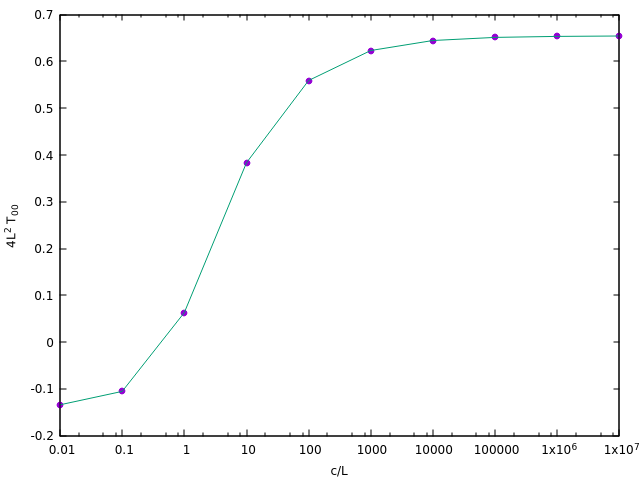
\includegraphics[height=0.4\textheight]{T00}
  \caption{The dependence on $\frac{c}{L}$ of $4L^2T_{00}$}\label{plotex1d}
\end{figure}






